% !TEX TS-program = xelatex

\chapter{Symbolic modeling with Julia Plasm}
\label{chapt:5}

Symbolic modeling is a semantic approach to knowledge representation and processing. A  symbolic approach to design with the aim of representing information and computation uses names to define the meaning of represented knowledge explicitly. The geometric knowledge is described here by Julia's names, which are chosen suitably for functionals, functions, formal and actual parameters, and finally for objects, fields, classes, attributes, methods, relations, etc. In this chapter, we give many examples of high-level Plasm programming, from topological, linear, and affine operators, to geometric mapping of complexes and grids to generate linearized approximation of curved manifold of intrinsic dimensions 1, 2, and 3. i.e., depending on such number of parameters; say, curves, surfaces, thin, and bulk solids.



\section{ Primitive generators}\label{sect:5-1}

Here, we introduce both single objects and aggregates of cells, typically by grid and mesh generators, resulting in a single |Hpc| value after the evaluation.


\subsection*{Higher order and partial functions}\label{sect:5-1-0}

As we have already seen in Section \ref{}, Julia |Plasm| is higher-level since allows for function that take functions as argument and/or may return a function value.  All functions are objects of Julia |Function| type. As objects (holding a reference to the function code), can be assigned to a name (identifier).

\begin{definition}[Function order] The \emph{order} of an object of |Function| type is the number of applications to actual parameters needed to return the ultimate actual value,  not a partial function value (needing further parameters).
\end{definition}

\begin{coding}[\sf  INTERVALS(size::Numrber)(n::Int)] In this example we show a second-order function (requiring two applications) that generates a 1D complex made by |n| line segments of total given |size| length.
\begin{lstlisting}[language=JuliaLocal, style=julia, mathescape=true]
segments = INTERVALS(10::Number)(4::Int)		#=
Hpc(MatrixNd(2), Geometry([[0.0], [2.5], [5.0], [7.5], [10.0]], hulls=[[1, 2], [2, 3], [3, 4], [4, 5]]))		=#
\end{lstlisting}
Note that |segments| value is 1D since its 11 vertices have one coordinate. 
\end{coding}


\begin{coding}[\sf  QUOTE(measures::Array{Number})]\
The formal parameter is an array of signed numbers.
\begin{lstlisting}[language=JuliaLocal, style=julia, mathescape=true]
two_aligned_segments = QUOTE([1,-2.5,1])			#=
Hpc(MatrixNd(2), Geometry([[0.0], [1.0], [3.5], [4.5]], hulls=[[1, 2], [3, 4]]))	=#
\end{lstlisting}
Positive numbers denote solid intervals of a given size; negative numbers denote hollow space, i.e., displacement of following segments. Successive negative numbers are allowed.\end{coding}


\begin{coding}[\sf  Q(measure::Number)]\
The formal parameter is a signed number. 
\begin{lstlisting}[language=JuliaLocal, style=julia, mathescape=true]
segment = Q(10)
Hpc(MatrixNd(2), Geometry([[0.0], [10.0]], hulls=[[1, 2]]))
\end{lstlisting}
A single |segment| of given size.
\end{coding}


\subsection*{Single convex cell}\label{sect:5-1-1}

Julia |Plasm| contains a great library of generator functions of very simple objects made by a single convex cell, and completely specified by its set of vertices only. 
Few examples follow; Other examples can be extracted or generated by the user looking at file |src/fenvs.jl|, including the Platonic solids. The multidimensional $d$-permutaheron is generated in Coding \ref{4-2-permutahedron}. 

\begin{coding}[\sf  CUBOID(size)]\
Multidimensional cuboid with |sizes::Vector{Number}|.
\begin{lstlisting}[language=JuliaLocal, style=julia, mathescape=true]
CUBOID([1])			#=
Hpc(MatrixNd(2), Hpc(MatrixNd(2), Geometry([[0.0], [1.0]], hulls=[[1, 2]]))) =#

CUBOID([1,2])			#=
Hpc(MatrixNd([[1.0, 0.0, 0.0], [0.0, 1.0, 0.0], [0.0, 0.0, 2.0]]), Hpc(MatrixNd(3), Geometry([[0.0, 0.0], [1.0, 0.0], [1.0, 1.0], [0.0, 1.0]], hulls=[[1, 2, 3, 4]]))) =#

CUBOID([1,2,3])			#=
Hpc(MatrixNd([[1.0, 0.0, 0.0, 0.0], [0.0, 1.0, 0.0, 0.0], [0.0, 0.0, 2.0, 0.0], [0.0, 0.0, 0.0, 3.0]]), Hpc(MatrixNd(4), Geometry([[0.0, 0.0, 0.0], [1.0, 0.0, 0.0], [0.0, 1.0, 0.0], [1.0, 1.0, 0.0], [0.0, 0.0, 1.0], [1.0, 0.0, 1.0], [0.0, 1.0, 1.0], [1.0, 1.0, 1.0]], hulls=[[1, 2, 3, 4, 5, 6, 7, 8]]))) =#

CUBOID([1,2,3,4])			#=
Hpc(MatrixNd([[1.0, 0.0, 0.0, 0.0, 0.0], [0.0, 1.0, 0.0, 0.0, 0.0], [0.0, 0.0, 2.0, 0.0, 0.0], [0.0, 0.0, 0.0, 3.0, 0.0], [0.0, 0.0, 0.0, 0.0, 4.0]]), Hpc(MatrixNd(5), Geometry([[0.0, 0.0, 0.0, 0.0], [1.0, 0.0, 0.0, 0.0], [0.0, 1.0, 0.0, 0.0], [1.0, 1.0, 0.0, 0.0], [0.0, 0.0, 1.0, 0.0], [1.0, 0.0, 1.0, 0.0], [0.0, 1.0, 1.0, 0.0], [1.0, 1.0, 1.0, 0.0], [0.0, 0.0, 0.0, 1.0], [1.0, 0.0, 0.0, 1.0], [0.0, 1.0, 0.0, 1.0], [1.0, 1.0, 0.0, 1.0], [0.0, 0.0, 1.0, 1.0], [1.0, 0.0, 1.0, 1.0], [0.0, 1.0, 1.0, 1.0], [1.0, 1.0, 1.0, 1.0]], hulls=[[1, 2, 3, 4, 5, 6, 7, 8, 9, 10, 11, 12, 13, 14, 15, 16]]))) =#
\end{lstlisting}
Cuboids of given sizes. Of course, the unit hypercube in $\E^6$ has |size = [1,1,1,1,1,1]|. 
\end{coding}

The |Plasm| coding of the “icosphere”, polyhedral approximation of the 2-sphere obtained by subdividing the |ICOSAHEDRON()| surface is given here, starting from the Platonic solid. The generation method is extremely simple. We obtain the vertices at step $i+1$ by adding to the vertices at step $i$ those obtained by subdivision of all edges. Ma make use of theHpc structure and the Lar structure.


\begin{coding}[\sf  ICOSPHERE(seed::Hpc)::Hpc]\
First we generate the cell complex of the input |obj| using the |LAR| combinator, then for each edge we compute the mean point, then we aggregate to the old vertices the new ones, scaled by the factor |r1/s1| built with the distance from |[0,0,0]| center of both models.
\begin{lstlisting}[language=JuliaLocal, style=julia, mathescape=true]
function ICOSPHERE(obj::Hpc)::Hpc
   W  = LAR(obj).V
   EV = LAR(obj).C[:EV]
   W  = [W[:,k] for k=1:size(W,2)]
   V  = [(W[v1]+W[v2])./2 for (v1,v2) in EV]
   r1 = sqrt(sum(W[1].^2))
   s1 = sqrt(sum(V[1].^2))
   CONVEXHULL([W; V*(r1/s1)]);
end
\end{lstlisting}
Finally, the |[W; V*(r1/s1)]::Vector{Vector{Float64}}| made by old vertices and by new scaled ones is given to the operator |CONVEXHULL| that transforms such a |Vector| of point (|Vector{Float64}|) in their geometric \emph{convex hull}.
Just remember that such polyhedra are convex sets, hence they have a \emph{single} (convex) cell. \begin{lstlisting}[language=JuliaLocal, style=julia, mathescape=true]
out0 = ICOSAHEDRON();   VIEW(out0)
out1 = ICOSPHERE(out0); VIEW(out1)
out2 = ICOSPHERE(out1); VIEW(out2)
out3 = ICOSPHERE(out2); VIEW(out3)
...		
\end{lstlisting}
Successive approximations of icosphere with 12, 42, 162, 600, etc., vertices.
Let’s remark the extreme simplicity of such polyhedral generations.
\end{coding}

\begin{figure}[htbp] %  figure placement: here, top, bottom, or page
   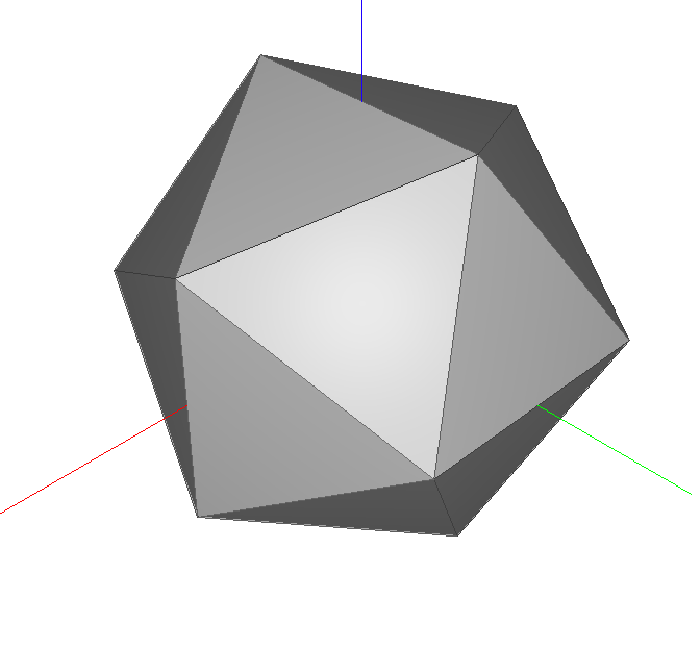
\includegraphics[width=0.34\linewidth]{chapter-05/figs/icosphere0}%
   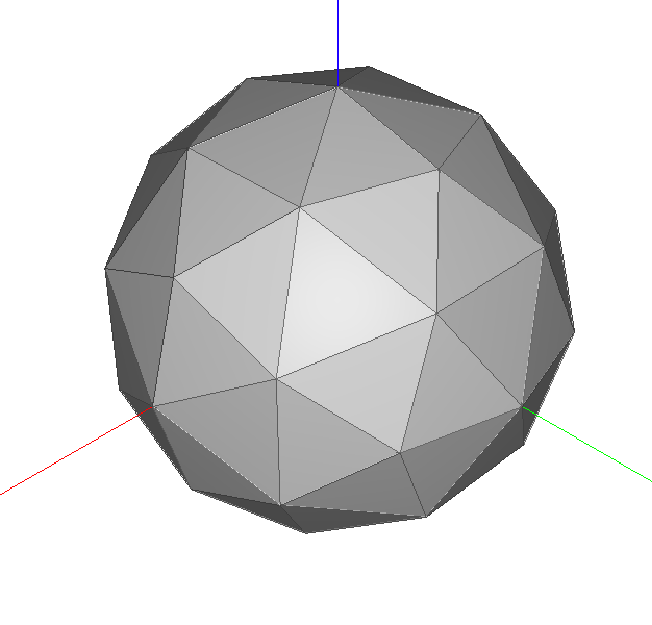
\includegraphics[width=0.33\linewidth]{chapter-05/figs/icosphere1}%
   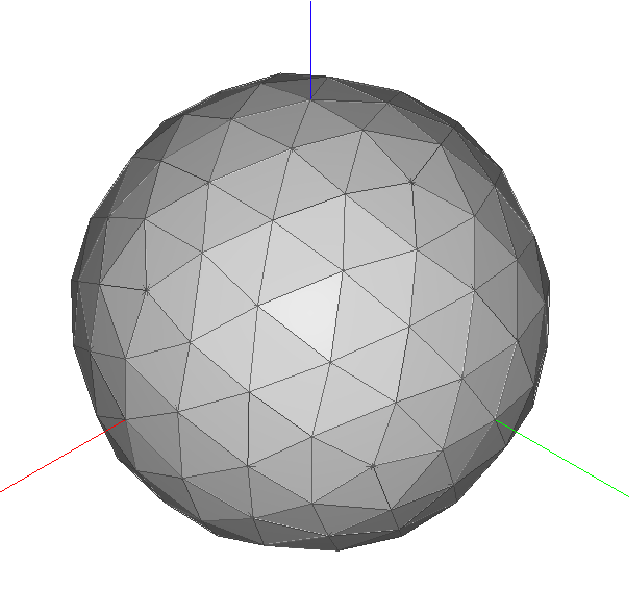
\includegraphics[width=0.325\linewidth]{chapter-05/figs/icosphere2}%
\hfill
\caption{(a) Icosahedron; (b) icosphere with 42 vertices; (c)  icosphere with 162 vertices. }
\label{5:icospheres}
\end{figure}



\subsection*{Multiple cell objects}\label{sect:5-1-1}


The functions |INTERVALS| or |QUOTE| may be used to create many types and patterns of grid geometries.

\begin{script}[Building frame]\
First we give the main dataset of a building frame, by “quoting” the side measures of 2D design plan:
\begin{lstlisting}[language=JuliaLocal, style=julia, mathescape=true]
# Longitudinal trusses
Y = QUOTE([0.3, -6, 0.3, -6, 0.3])
# transverse beams
X = QUOTE([0.3, -3, 0.3, -4.2, 0.3, -3, 0.3])
# vertical measurements
Z = QUOTE([3,0.3])
\end{lstlisting}
Then, an alternate set of |INTERVALS| vector parameters are generated by Julia broadcast |.*| of the scalar |-1|, in order to invert all the signs.
\begin{lstlisting}[language=JuliaLocal, style=julia, mathescape=true]
X1 = QUOTE([0.3, -3, 0.3, -4.2, 0.3, -3, 0.3].* -1)
Y1 = QUOTE([0.3, -6, 0.3, -6, 0.3].*-1)
Z1 = QUOTE([3,-0.3].*-1)
\end{lstlisting}
Below, the 3D |frame| subsystems are generated. They are the $C_3$ basis of a local cellular complex. Note the variation pattern at |trusses1|.
\begin{lstlisting}[language=JuliaLocal, style=julia, mathescape=true]
# Cartesian product
pillars = COLOR(RED)(X*Y*Z);
trusses = COLOR(YELLOW)(X*Y1*Z1);
trusses1 = COLOR(YELLOW)(X1*Y*QUOTE([-2.7,0.6]));
floorslab = COLOR(GREEN)(X1*Y1*Z1);
\end{lstlisting}
Finally, the sub-complexes of 3D cells are aggregated in a single |Plasm| complex using the |STRUCT| combinator discussed in the next session. Let us note that in this example all the aggregated models live in the same reference frame.
\begin{lstlisting}[language=JuliaLocal, style=julia, mathescape=true]
frame = STRUCT(pillars, trusses, trusses1, floorslab);
VIEW(frame, Dict("background_color"=>WHITE))
\end{lstlisting}
\end{script}


\begin{figure}[htbp] %  figure placement: here, top, bottom, or page
   \sidecaption[t]
   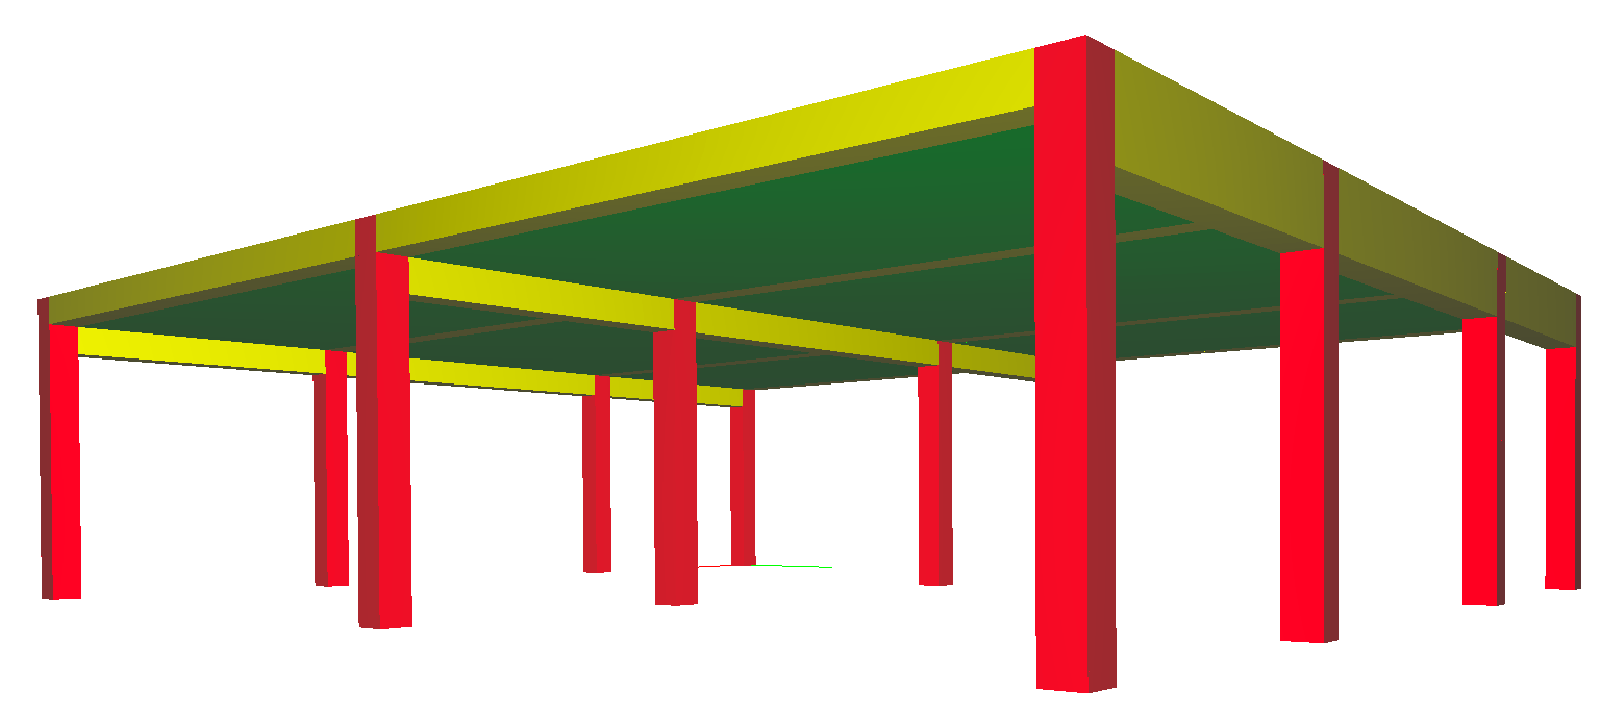
\includegraphics[width=\linewidth]{chapter-05/figs/frame1} 
   \caption{\sf frame = STRUCT(pillars, trusses, trusses1, floorslab);}.}
   \label{fig:example}
\end{figure}
\subsection*{Assembly combinator {\sf STRUCT}}\label{sect:5-1-1}

We have already come across the |STRUCT| function, one of more important |Plasm| operators. In particular, we already know that |STRUCT| is used to assembly geometric objects into a single object. In Julia |Plasm| both the input and the output objects are of recursive |Hpc| type.

In geometric modeling of complex assemblies the geometric and graphics
programmer makes wide use of the \emph{hierarchical scene
graphs}~\cite{Wernecke:94:TIM,Sowizral:2000:J3DAPI} or hierarchical
structures~\cite{Gaskins92}, where sub-assemblies are defined in \emph{local}
coordinates, and are transformed into the coordinate frame of the
output assembly by explicitly using proper coordinate
transformations.  

It is worth noting that such “modeling transformations" --- as they are called in graphical systems --- are left entirely to programmer's responsibility.  


\begin{figure}[htbp] %  figure placement: here, top, bottom, or page
   \sidecaption[t]
   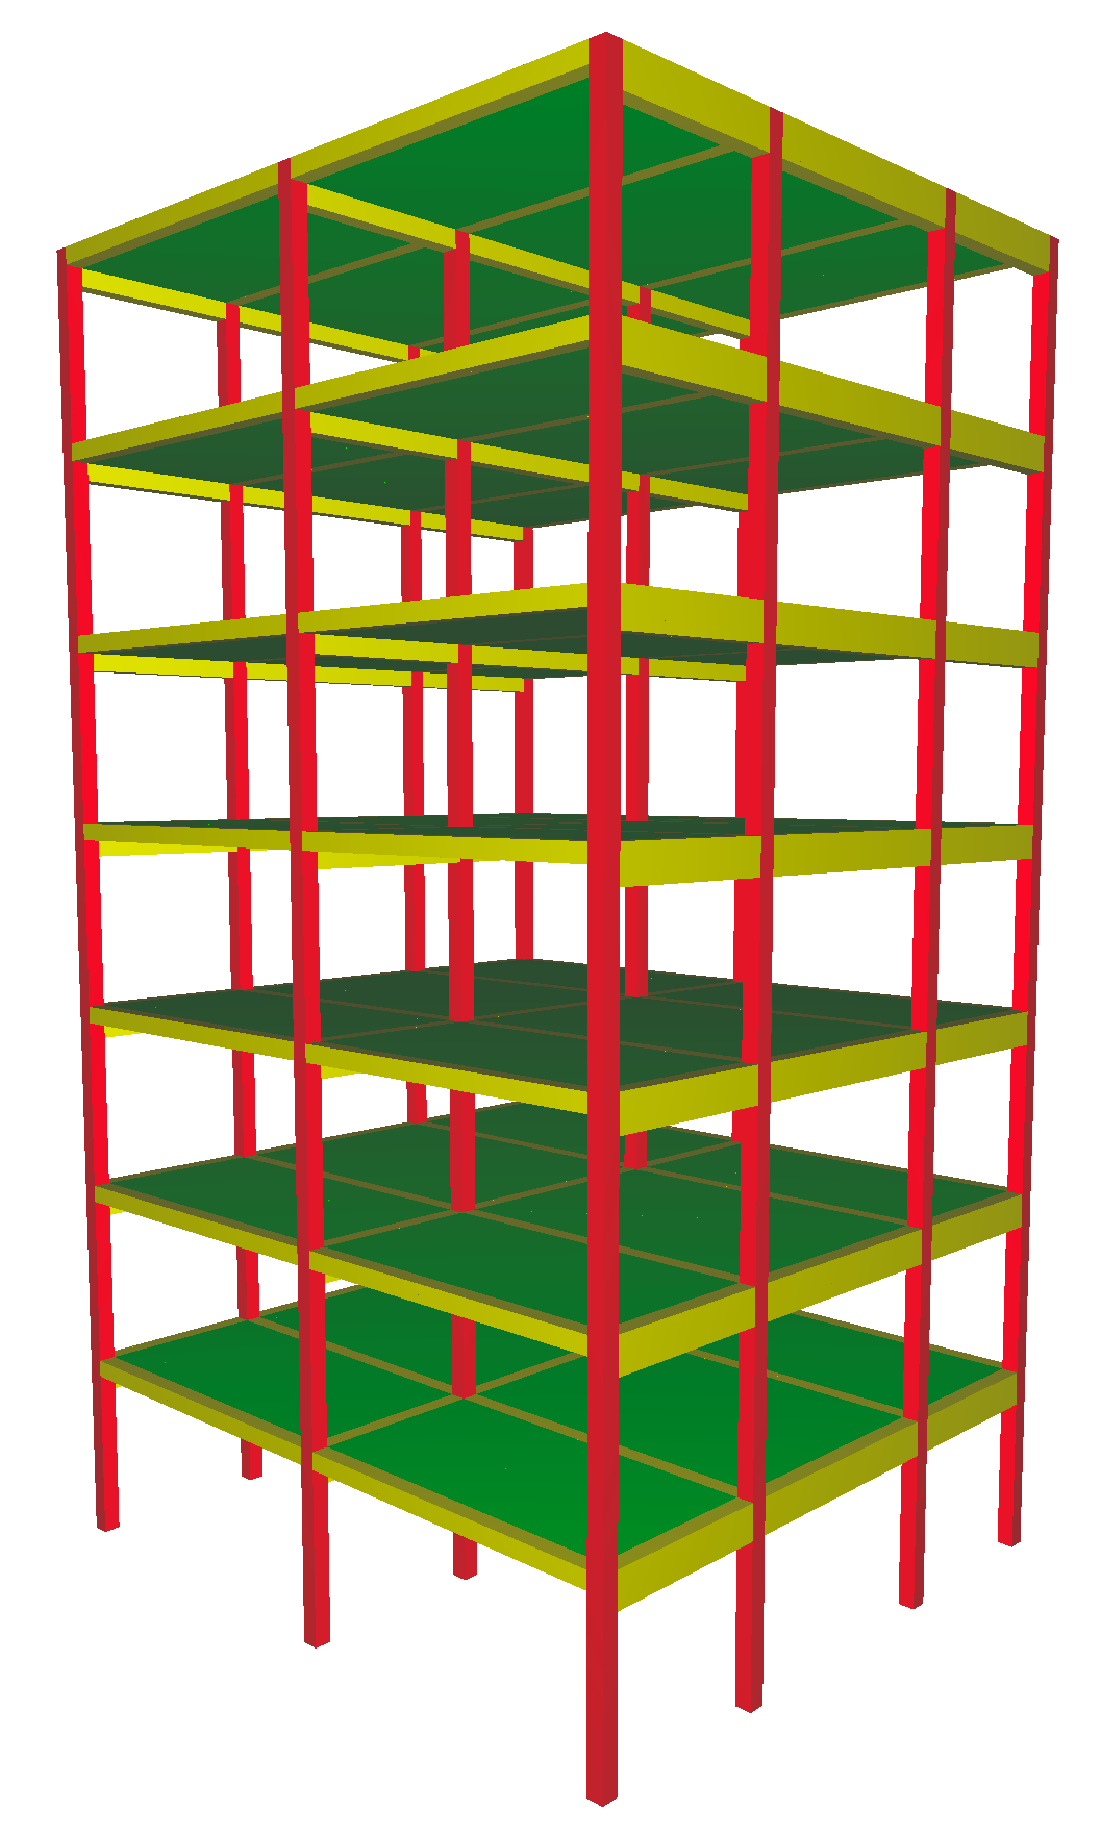
\includegraphics[width=0.6\linewidth]{chapter-05/figs/skeleton1} 
   \caption{\sf skeleton = STRUCT(NN(7)([frame, T(3)(3.3)])));}.}
   \label{fig:5:1:skeleton}
\end{figure}

\begin{coding}[Building skeleton]\label{5:1:skeleton}
We assemble here a building skeleton model, by creating a |STRUCT| assembly generated by |n=7| instances of the Julia |Vector| made by the |Hpc| value |frame| and by the |MatrixNd| value |T(3)(3.3)| producing a translation in $z$ direction.
\begin{lstlisting}[language=JuliaLocal, style=julia, mathescape=true]
skeleton = STRUCT(NN(7)([frame, T(3)(3.3)]));
VIEW(skeleton, Dict("background_color"=>WHITE)
\end{lstlisting}
\end{coding}

Here the |STRUCT| semantics is very clear: the evaluated subexpression |NN(7)([frame, T(3)(3.3)])| is an array of type |Vector{Union{Hpc, MatrixNd}}| and contain 14 item with alternating types.  When |STRUCT| is evaluted on this vector, an |Hpc| node is generated, whose |MatrixNd| field contains a $4\times 4$ identity matrix, and the |childs| vector contains the reference to the first item of 


\subsection*{Alignment aggregators {\sf TOP, BOTTOM, LEFT, RIGTH}}\label{sect:5-1-1}


In the present section we discuss some simplified assembly operators, where the
coordinate transformations are computed automatically by the language.

|Plasm| has some predefined binary functions used to locate two complexes with respect each other.  In particular,
the second argument of such functions will be positioned either
|TOP| the first one, or |ABOVE|, or |LEFT|, or
|RIGHT|, or |UP|, or |DOWN|, respectively,
according to the alignment semantics given below.

Such relative positioning allows
for an easy construction of complex assemblies, without taking into account the local coordinate frames where the
sub-assemblies are defined.  In this way we avoid applying affine transformations as it is
conversely needed in hierarchical scene graphs.

\begin{coding}[alternate method for vertical aggregation]\
\begin{lstlisting}[language=JuliaLocal, style=julia, mathescape=true]
multifloor(model,n) = STRUCT(INSR(TOP)(N(n+1)(model))) #=
multifloor (generic function with 1 method)		  	   =#
VIEW(multifloor(frame,7))
\end{lstlisting}
The object generated here is equal to the |skeleton| model of Figure \ref{fig:5:1:skeleton}. 
\end{coding}

|TOP| is a binary function of two |Hpc| models that creates their vertical aggregation.
Any binary function is transformed in $n$-ary by the second order operator |INSR| (for \emph{insert right}). |INSR| is applied first to the operator argument to make $n$-ary, then to the list of objects the operator apply to.

|N(n)(value::Any)| is a |Plasm| function called $\#$ in classic |PLaSM|, that returns a list of |n| instances of |value|. 

\begin{definition}[Primitive {\sf ALIGN} function.]
Every pair of polyhedral complexes may be aligned along any given subset of coordinates by using the primitive binary function |ALIGN|. Such a second-order operator must be applied to a sequence of triples which define a specialized behavior for each affected coordinate.
\end{definition}

Each alignment directive along a coordinate must belong to the set
\[
[1,n] \times \{ |MIN,MED,MAX,K($\alpha$)|\} 
\times \{ |MIN,MED,MAX,K($\alpha$})|\}
\]
where |$\alpha$::Number|, used to align on a given coordinate. The resulting specialized operator is then applied to a pair of |Hpc| values, and returns a single |Hpc|.  Use examples following the |ALIGN| combinator for other operators' definitions.
\begin{lstlisting}[language=JuliaLocal, style=julia, mathescape=true]
TOP = ALIGN([[3, MAX, MIN], [1, MED, MED], [2, MED, MED]])
BOTTOM = ALIGN([[3, MIN, MAX], [1, MED, MED], [2, MED, MED]])
LEFT = ALIGN([[1, MIN, MAX], [3, MIN, MIN]])
RIGHT = ALIGN([[1, MAX, MIN], [3, MIN, MIN]])
UP = ALIGN([[2, MAX, MIN], [3, MIN, MIN]])
DOWN = ALIGN([[2, MIN, MAX], [3, MIN, MIN]])
# 294 (generic function with 1 method)
\end{lstlisting}


\begin{figure}[htbp] %  figure placement: here, top, bottom, or page
   \sidecaption[t]
   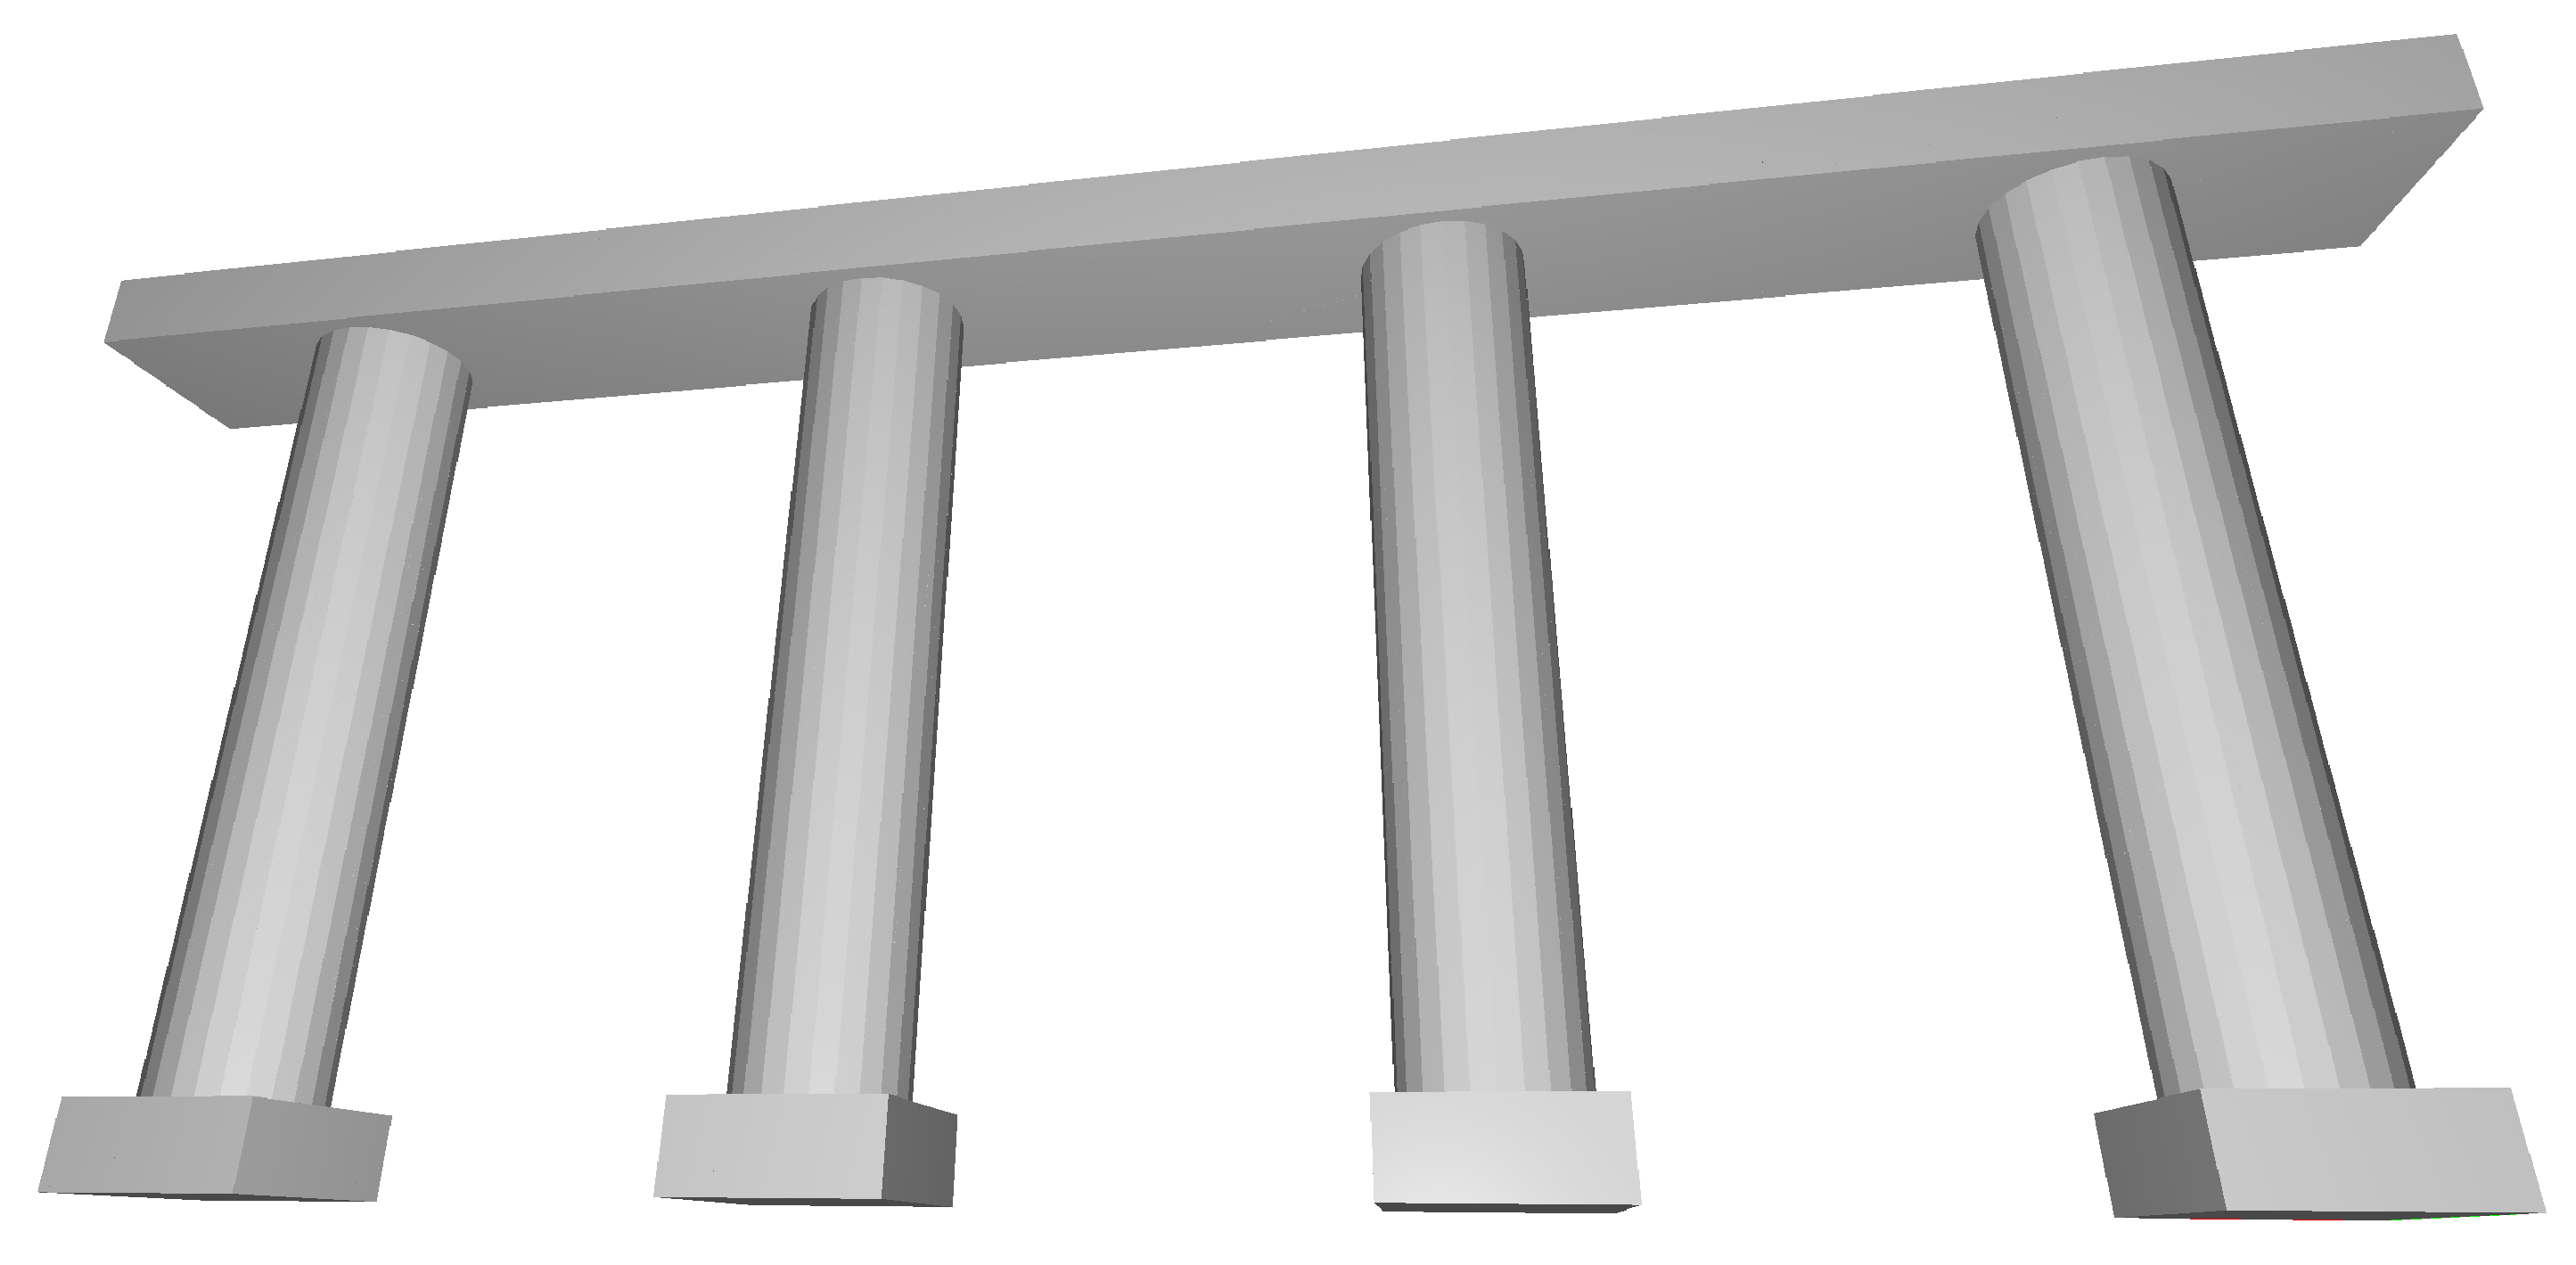
\includegraphics[width=\linewidth]{chapter-05/figs/fourcolumns} 
   \caption{\sf skeleton = STRUCT(NN(7)([frame, T(3)(3.3)])));}.}
   \label{fig:5:1:fourcolumns}
\end{figure}

\begin{coding}\
A very simplified view of a column is built here, to show the use of the |INSR(TOP)| and |INSR(RIGHT)| functions applied to a list of geometric object, each given in its local coordinate system:
\begin{lstlisting}[language=JuliaLocal, style=julia, mathescape=true]
function Column(r,h)
   basis = CUBOID([ 2*r*1.2, 2*r*1.2, h/12.0 ]) 
   trunk = CYLINDER([ r, (10.0/12.0)*h ])(12)
   capital = CUBOID([ 2*r*1.2, 2*r*1.2, h/12.0 ])
   beam = S(1)(3)(capital) 
   return INSR(TOP)([basis,trunk,capital,beam])
end
# Column (generic function with 2 methods)
\end{lstlisting}

\begin{lstlisting}[language=JuliaLocal, style=julia, mathescape=true]
function ColRow(N,r,h)
   col = Column(r,h)
   columnlist = [col for k in 1:N+1]
   return INSR(RIGHT)(columnlist)
end
# ColRow (generic function with 2 methods)
\end{lstlisting}

\begin{lstlisting}[language=JuliaLocal, style=julia, mathescape=true]
VIEW(ColRow(4,1.,12.), Dict( => WHITE))
\end{lstlisting}
The generated model is displayed in Figure \ref{}
\end{coding}



\begin{figure}
\begin{minipage}[t]{0.571\linewidth}
	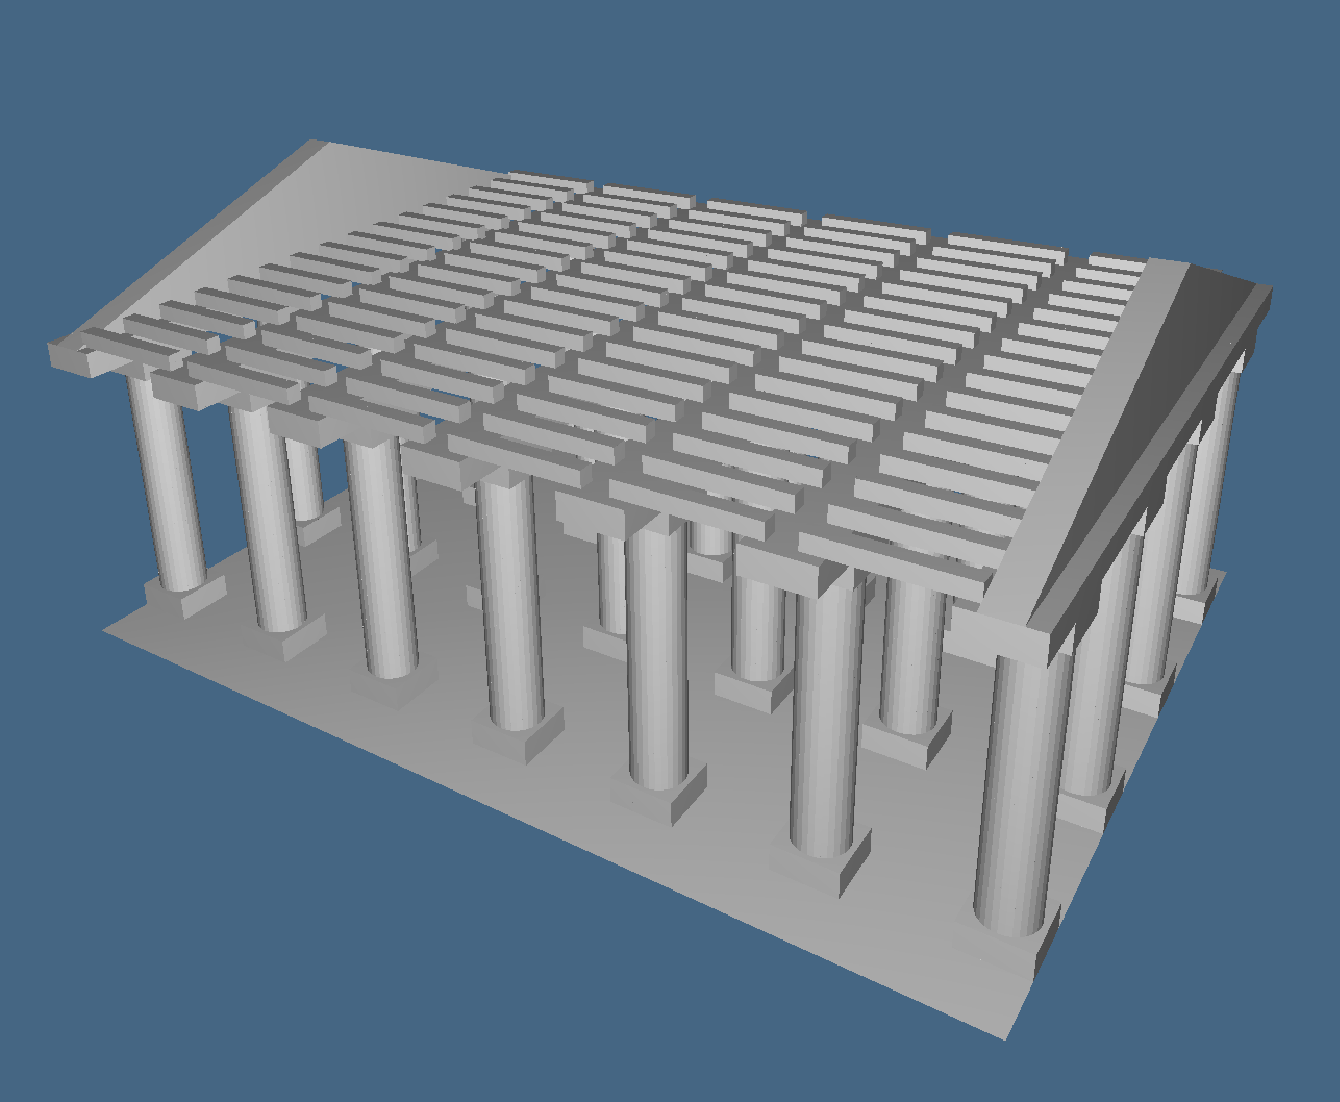
\includegraphics[width=\linewidth]{chapter-05/figs/temple-01}%

		\vspace{-1mm}
	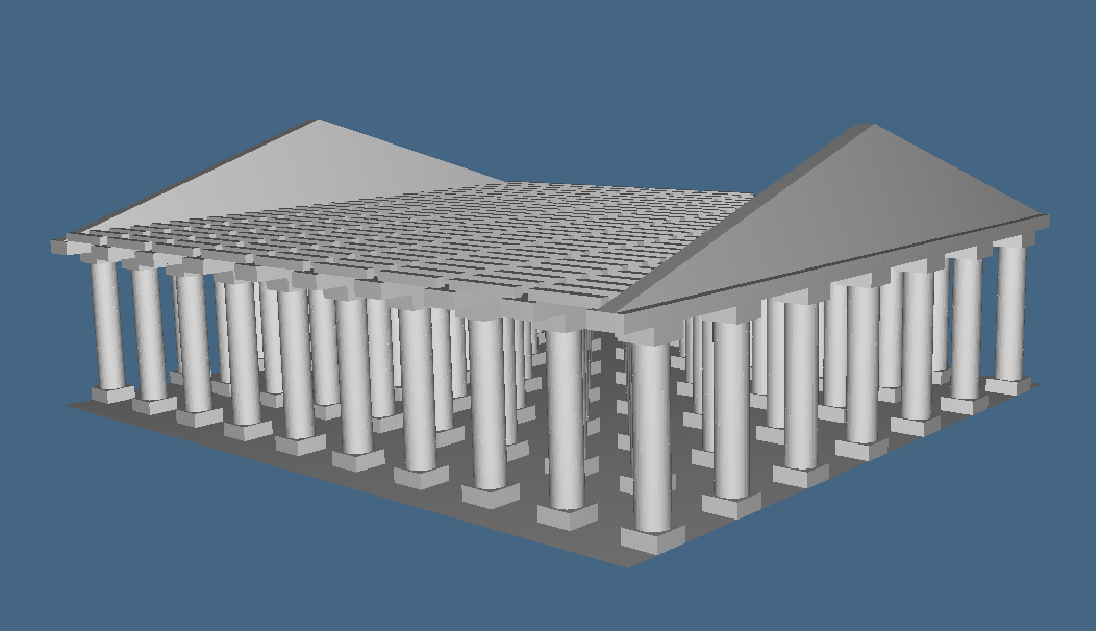
\includegraphics[width=\linewidth]{chapter-05/figs/temple-02}
	%\label{fig:example}
\end{minipage}%
\begin{minipage}[t]{0.429\linewidth}
	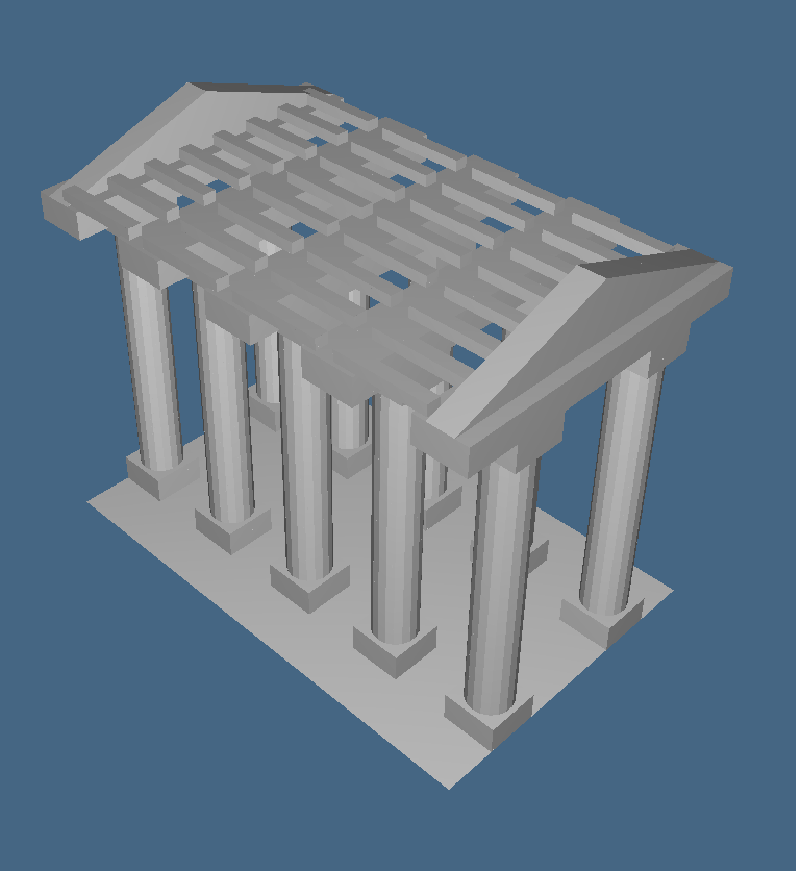
\includegraphics[width=\linewidth]{chapter-05/figs/temple-03}
\caption{A fully parameterized {\sf Temple()} function, where several parameters are linked to each other by algebraic equations. Let’s note the number of side and front columns, and their relations with column height and gable width. The whole function code is about 15 rows.}
\end{minipage}
\end{figure}




\section{ Plasm topological operators}\label{sect:5-2}

For the sake of simplicity, we start here our presentation of programming through  topological operators by discussing with one of simplest example models, the |Lar| numbered version of the 3-cube of side 1. Both the vector font of text and its integrated display with the object are by |Plasm| package.  Such integration with text was of invaluable utility in algorithm development.

First, in this model we have a 3D chain complex (see section~\ref{sect:3-3-2}) with 
one 3-cell, 6 faces (2-cells |FV|), 12 edges (1-cells |EV|), and 8 vertices (0-cells |V|).

\begin{figure}[htbp] %  figure placement: here, top, bottom, or page
   \sidecaption[t]
   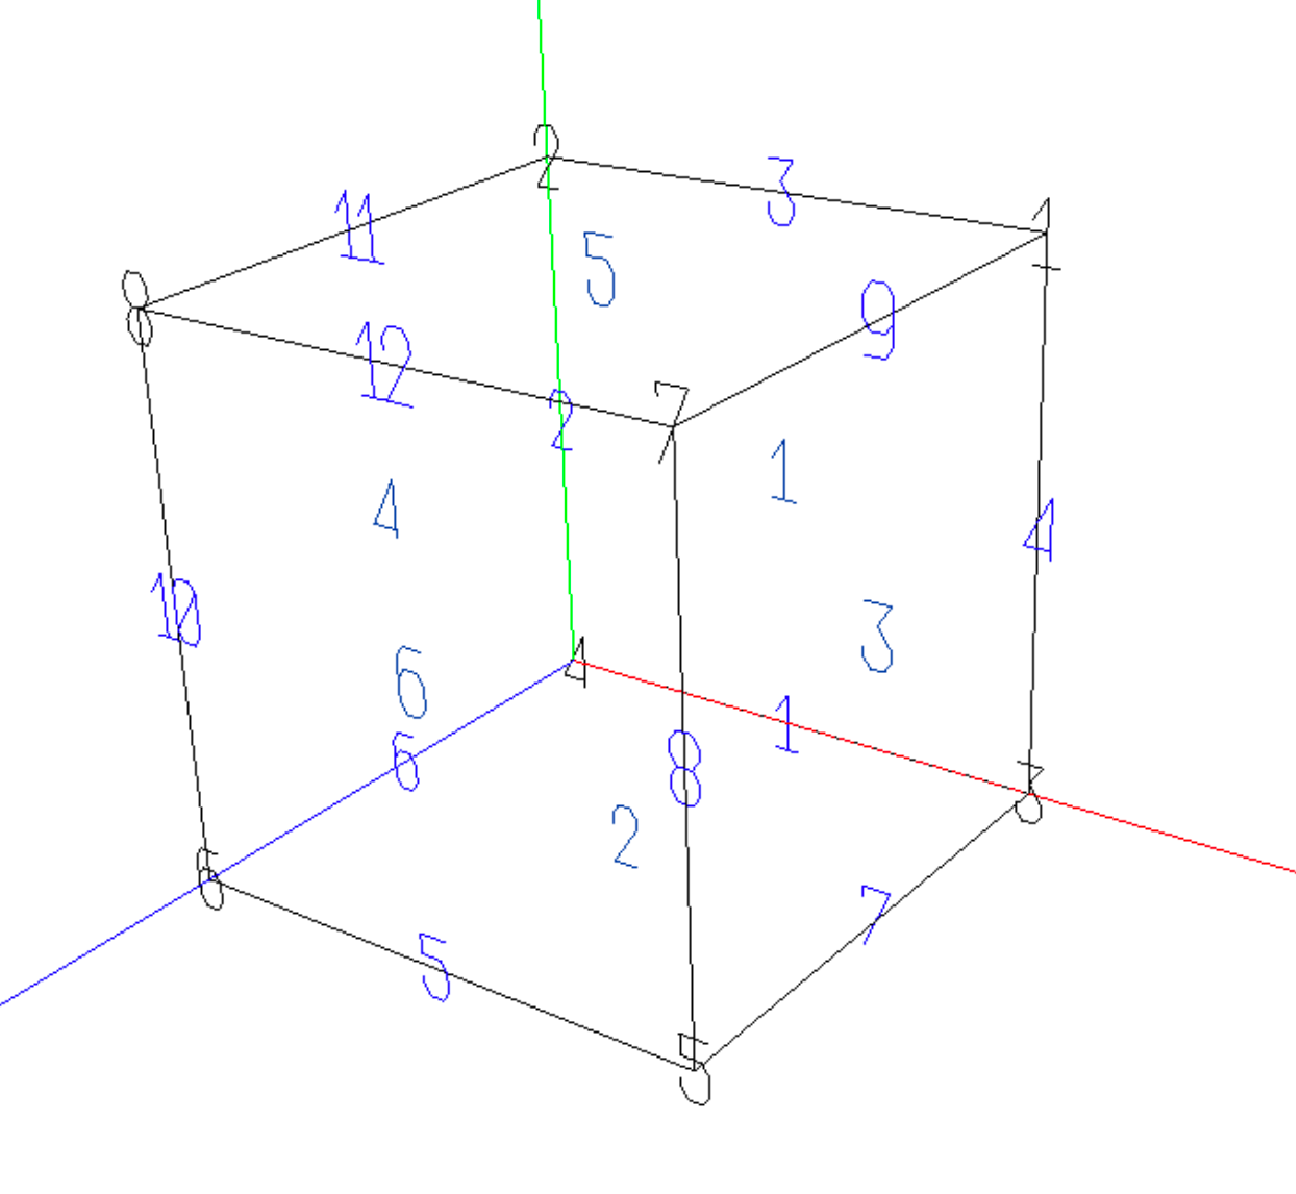
\includegraphics[width=0.5\linewidth]{chapter-05/figs/cube} 
   \caption{The numbered unit 3-cube cellular complex. 
   The ordinal numbers  for vertices, edges and faces are set at the middle of each 1-, 2-, and 3-cell. Note that the indexes have lexicographic and not geometric order (say, clockwise or counterclockwise), but this is not a constraint. }
   \label{fig:5:1:cube}
\end{figure}
The reader is instructed to check for comparison the following dataset with the Figure~\ref{fig:5:1:cube}. In general, the cell indices are unordered.
\begin{lstlisting}[language=JuliaLocal, style=julia, mathescape=true]
LAR(CUBE(1))		#=
Lar(3, 3, 8, [1.0 0.0 … 1.0 0.0; 1.0 1.0 … 1.0 1.0; 0.0 0.0 … 1.0 1.0], Dict{Symbol, AbstractArray}(:CV => [[1, 2, 3, 4, 5, 6, 7, 8]], :FV => [[1, 2, 3, 4], [3, 4, 5, 6], [1, 3, 5, 7], [2, 4, 6, 8], [1, 2, 7, 8], [5, 6, 7, 8]], :EV => [[3, 4], [2, 4], [1, 2], [1, 3], [5, 6], [4, 6], [3, 5], [5, 7], [1, 7], [6, 8], [2, 8], [7, 8]])) =#
\end{lstlisting}

Consider the three entities |V, E, F| of solid objects' boundary representations (|B-rep|).
Therefore, we have three binary adjacency relations, VV, EE, and FF, and six binary incidence relations, VE, VF, EV, EF, FV, and FE. The latter group is well-known to topologists, while software engineers mainly use the former to design efficient data structures for solid modeling.

We introduce here a new entity, |C|, to denote solid cells in 3D, and two new incidence relations, |CF, FC|, used by our |Lar| (Linear Algebraic Representation) to build the |B-reps| itself and the Boolean Algebras of solids. The relations |CV, VC| are directly used by the |Hpc| representation.

\subsection{Incidence operators}\label{sect:5-2-1}

The “unevaluated” |Lar| representation is based on |FV| and |EV| (other than on the |V| matrix of vertex coordinates) where the 2- and 1-cells are given as unordered lists of 0-cells’s indices, i.e., as chains of vertices, and stored in Julia by the type |Chains = Vector{Vector{Int64}}|.
\begin{lstlisting}[language=JuliaLocal, style=julia, mathescape=true]
EV = LAR(CUBE(1)).C[:EV];		#=
12-element Vector{Vector{Int64}}:	
[[3, 4], [2, 4], [1, 2], [1, 3], [5, 6], [4, 6], [3, 5], [5, 7], [1, 7], [6, 8], [2, 8], [7, 8]]		=#
FV = LAR(CUBE(1)).C[:FV]		#=
6-element Vector{Vector{Int64}}:
[[1, 2, 3, 4], [3, 4, 5, 6], [1, 3, 5, 7], [2, 4, 6, 8], [1, 2, 7, 8], [5, 6, 7, 8]]		=#
\end{lstlisting}

When represented as sparse binary matrices, the |FV| and |EV| relations, as such defined as subsets of the Cartesian products |F$\times$V| and |E$\times$V|, allow for an easy algebraic computation of [|FE|], as we see in the following, as well for their transposed matrices |[FV]$^\top$= [VF]|,  |EV|$^\top$, and [|FE|]$^\top$.

The sparse matrix is of type
|ChainOp = SparseArrays.SparseMatrixCSC{Int8, Int64}|, where |CSC| stands for |Compressed Sparse Column|, generated by the |lar2cop| function, where |cop| stands for |ChainOp|:

\begin{lstlisting}[language=JuliaLocal, style=julia, mathescape=true]
KEV = lar2cop(EV)
12×8 SparseArrays.SparseMatrixCSC{Int8, Int64} with 24 stored entries:
 ⋅  ⋅  1  1  ⋅  ⋅  ⋅  ⋅
 ⋅  1  ⋅  1  ⋅  ⋅  ⋅  ⋅
 1  1  ⋅  ⋅  ⋅  ⋅  ⋅  ⋅
 1  ⋅  1  ⋅  ⋅  ⋅  ⋅  ⋅
 ⋅  ⋅  ⋅  ⋅  1  1  ⋅  ⋅
 ⋅  ⋅  ⋅  1  ⋅  1  ⋅  ⋅
 ⋅  ⋅  1  ⋅  1  ⋅  ⋅  ⋅
 ⋅  ⋅  ⋅  ⋅  1  ⋅  1  ⋅
 1  ⋅  ⋅  ⋅  ⋅  ⋅  1  ⋅
 ⋅  ⋅  ⋅  ⋅  ⋅  1  ⋅  1
 ⋅  1  ⋅  ⋅  ⋅  ⋅  ⋅  1
 ⋅  ⋅  ⋅  ⋅  ⋅  ⋅  1  1
\end{lstlisting}


\begin{lstlisting}[language=JuliaLocal, style=julia, mathescape=true]
KFV = lar2cop(FV)
6×8 SparseArrays.SparseMatrixCSC{Int8, Int64} with 24 stored entries:
 1  1  1  1  ⋅  ⋅  ⋅  ⋅
 ⋅  ⋅  1  1  1  1  ⋅  ⋅
 1  ⋅  1  ⋅  1  ⋅  1  ⋅
 ⋅  1  ⋅  1  ⋅  1  ⋅  1
 1  1  ⋅  ⋅  ⋅  ⋅  1  1
 ⋅  ⋅  ⋅  ⋅  1  1  1  1
\end{lstlisting}

\begin{remark}
It is essential to note that |KEV: V$\to$E| and |KFV: V$\to$F| are linear operators between the linear subspaces |V|, |E|, |F| of 0-, 1-, 2-chains. |EV| and |FV| represent the elementary bases of chain subspaces |E|, |F| in terms of |V| basis. 
\end{remark}

For the sake of clarity, it may be useful to update the mathematical notation of “chain complex” (see \ref{sect:3-3-2}), given again below for user sake, with our data structure notations. For the sake of simplicity, we often drop the |K| from names, and use |EV|, |FE|, and |CF| with meaning depending on the context.

\[ 
C_\bullet = (C_p, \partial_p) := 
C_3 \ 
\substack{
\delta_2 \\
\longleftarrow \\[-1mm]
\longrightarrow \\
\partial_3 
}
\ C_2 \ 
\substack{
\delta_1 \\
\longleftarrow \\[-1mm]
\longrightarrow \\
\partial_2 
}
\ C_1 \ 
\substack{
\delta_0 \\
\longleftarrow \\[-1mm]
\longrightarrow \\
\partial_1 
}
\ C_0 
\quad\equiv\quad
C_3 \ 
\substack{
\textsf{\scriptsize CF}\\
\longleftarrow \\[-1mm]
\longrightarrow \\
\textsf{\scriptsize FC}
}
\ C_2 \ 
\substack{
\textsf{\scriptsize FE}\\
\longleftarrow \\[-1mm]
\longrightarrow \\
\textsf{\scriptsize EF}
}
\ C_1 \ 
\substack{ 
\textsf{\scriptsize EV}\\
\longleftarrow \\[-1mm]
\longrightarrow \\
\textsf{\scriptsize VE}
}
\ C_0 .
\] 

\begin{coding}[Algebraic computation of FE = $\delta_1$]
By now, the |FE| operator |E|$ \to $|F| is not yet known and must be computed and added to the |Lar| dataset, if needed. 
We may compute it algebraically by product of |FV| times |VE = EV$^\top$|.  Using the two  sparse matrices we have:
\begin{lstlisting}[language=JuliaLocal, style=julia, mathescape=true]
KFV * KEV'
6×12 SparseArrays.SparseMatrixCSC{Int8, Int64} with 48 stored entries:
 2  2  2  2  ⋅  1  1  ⋅  1  ⋅  1  ⋅
 2  1  ⋅  1  2  2  2  1  ⋅  1  ⋅  ⋅
 1  ⋅  1  2  1  ⋅  2  2  2  ⋅  ⋅  1
 1  2  1  ⋅  1  2  ⋅  ⋅  ⋅  2  2  1
 ⋅  1  2  1  ⋅  ⋅  ⋅  1  2  1  2  2
 ⋅  ⋅  ⋅  ⋅  2  1  1  2  1  2  1  2
\end{lstlisting}
The second term was transposed (|'|) to get compatibility (|size(KFV,2)==size(KEV’,1)|.
Note that each product term |(x$_{i,j}$)| represents the number of vertices in common between row $i$ and column $j$ of the two matrices (look at Figure \ref{fig:5:1:cube}).

This matrix must be filtered to remainder of |÷ 2| (integer division by two).
Thus, we get algebraically the binary matrix of the incidence relation |FE|:
\begin{lstlisting}[language=JuliaLocal, style=julia, mathescape=true]
KFE = KFV * KEV' .÷ 2
6×12 SparseArrays.SparseMatrixCSC{Int64, Int64} with 24 stored entries:
 1  1  1  1  ⋅  ⋅  ⋅  ⋅  ⋅  ⋅  ⋅  ⋅
 1  ⋅  ⋅  ⋅  1  1  1  ⋅  ⋅  ⋅  ⋅  ⋅
 ⋅  ⋅  ⋅  1  ⋅  ⋅  1  1  1  ⋅  ⋅  ⋅
 ⋅  1  ⋅  ⋅  ⋅  1  ⋅  ⋅  ⋅  1  1  ⋅
 ⋅  ⋅  1  ⋅  ⋅  ⋅  ⋅  ⋅  1  ⋅  1  1
 ⋅  ⋅  ⋅  ⋅  1  ⋅  ⋅  1  ⋅  1  ⋅  1
\end{lstlisting}

\begin{remark}
We like to remark that to setup the incidence data structures with this algebraic approach has the same space and time complexity than using standard data structures for solid modeling \cite{DBLP:journals/cad/DiCarloPS14}. Conversely, the aggregated queries for several entity items are much faster, since computable by a single Matrix-Vector, or even  Matrix-Matrix product.
\end{remark}
\begin{remark}
Let’s notice that the operator matrix |FE| for the 3D object |CUBE| has two nonzero on each column and four nonzeroes on each row, so implementing the incidence relation between faces and edges correctly.
\end{remark}



\subsection{Adiacency operators}\label{sect:5-2-1}

The adjacency relations, in our context, are the sparse symmetric matrices, i.e., 
|FV*VF|, |EV*VE|, and |EV*VE|. In this case we have, using our input sparse matrices |KFV| and |KEV| with transposition (if needed) for product compatibility:

\begin{lstlisting}[language=JuliaLocal, style=julia, mathescape=true]
A = KFV * KFV'; FF = (A - Diagonal(A)) .÷ 2
6×6 SparseMatrixCSC{Int64, Int64} with 24 stored entries:
 ⋅  1  1  1  1  ⋅
 1  ⋅  1  1  ⋅  1
 1  1  ⋅  ⋅  1  1
 1  1  ⋅  ⋅  1  1
 1  ⋅  1  1  ⋅  1
 ⋅  1  1  1  1  ⋅
\end{lstlisting}

The user should know that |Diagonal| is a generator function of the Julia Package |LinearAlgebra|. 

\begin{lstlisting}[language=JuliaLocal, style=julia, mathescape=true]
B = KEV * KEV'; EE = (B - Diagonal(B))
12×12 SparseMatrixCSC{Int8, Int64} with 48 stored entries:
 ⋅  1  ⋅  1  ⋅  1  1  ⋅  ⋅  ⋅  ⋅  ⋅
 1  ⋅  1  ⋅  ⋅  1  ⋅  ⋅  ⋅  ⋅  1  ⋅
 ⋅  1  ⋅  1  ⋅  ⋅  ⋅  ⋅  1  ⋅  1  ⋅
 1  ⋅  1  ⋅  ⋅  ⋅  1  ⋅  1  ⋅  ⋅  ⋅
 ⋅  ⋅  ⋅  ⋅  ⋅  1  1  1  ⋅  1  ⋅  ⋅
 1  1  ⋅  ⋅  1  ⋅  ⋅  ⋅  ⋅  1  ⋅  ⋅
 1  ⋅  ⋅  1  1  ⋅  ⋅  1  ⋅  ⋅  ⋅  ⋅
 ⋅  ⋅  ⋅  ⋅  1  ⋅  1  ⋅  1  ⋅  ⋅  1
 ⋅  ⋅  1  1  ⋅  ⋅  ⋅  1  ⋅  ⋅  ⋅  1
 ⋅  ⋅  ⋅  ⋅  1  1  ⋅  ⋅  ⋅  ⋅  1  1
 ⋅  1  1  ⋅  ⋅  ⋅  ⋅  ⋅  ⋅  1  ⋅  1
 ⋅  ⋅  ⋅  ⋅  ⋅  ⋅  ⋅  1  1  1  1  ⋅
\end{lstlisting}


\begin{lstlisting}[language=JuliaLocal, style=julia, mathescape=true]
C = KEV' * KEV; VV = (C - Diagonal(C))
8×8 SparseMatrixCSC{Int8, Int64} with 24 stored entries:
 ⋅  1  1  ⋅  ⋅  ⋅  1  ⋅
 1  ⋅  ⋅  1  ⋅  ⋅  ⋅  1
 1  ⋅  ⋅  1  1  ⋅  ⋅  ⋅
 ⋅  1  1  ⋅  ⋅  1  ⋅  ⋅
 ⋅  ⋅  1  ⋅  ⋅  1  1  
 ⋅  ⋅  ⋅  1  1  ⋅  ⋅  1
 1  ⋅  ⋅  ⋅  1  ⋅  ⋅  1
 ⋅  1  ⋅  ⋅  ⋅  1  1  ⋅
\end{lstlisting}



\subsection{Atomic decomposition}\label{sect:5-2-3}

Here we shortly recall the main aspects of algebraic topological computation with linear spaces of chains of cells (see section~\ref{}).

We start by remarking the implementation as sparse matrices of the two plus two \emph{boundary} |FE|, |EV|, and \emph{coboundary} operators |EF|, |VE| of the (co)chain complex between three linear spaces of chains and cochains (with identified standard bases) $C_2, C_1, C_0$, i.e., |FE|, |EV|, |V|.

To be able to perform quite any kind of 3D geometric computation in the broadest area of Solid and Geometric Modeling, in last years enlarged by multi-material patterns, we need a fourth 3-chain space $C_3$, i.e., a linear space of 3D solid chains.

\begin{definition}[Elementary cells]
We define elementary cells of a cellular $d$-complex the arrangement $X=\{X_p\}$ ($0\leq p\leq d$) of open connected $p$-cells generated by a given collection ${\cal S}$ of closed $(d-1)$-manifolds partitioning the Euclidean $d$-space, i.e., such that $\cup_p X_p = \E^d,  X_p \cap X_q = \emptyset$.
\end{definition}

\begin{definition}[Elementary chain bases]
We define $p$-chain basis of an arrangement $X({\cal S})$ of $E^d$ the set of singletons corresponding one-to-one to elementary $p$-cells of $X$. 
\end{definition}

\begin{remark}
A chain subspace $C_p$ is the powerset $\mathcal{2}^{X_p}$ of the set $X_p$. The chain space $C$ is the direct sum of chain subspaces $C_p$ ($0\leq p\leq d$). Every chain may be uniquely formed by sum (|mod 2|) of basis elements, and by product of a chain times a scalar in $\{0,1\}$.
\end{remark}


Using chain concepts, we discuss in the next chapters how to generate 3D solid models using a generalization of Constructive Solid Geometry (CSG), which is a modeling method used in computer graphics and CAD systems. CSG allows the development of complex 3D models by solid operations like regularized union, intersection, and difference, either on simple primitive shapes or by mixing closed boundary models.

In the next chapters, we discuss a similar but more powerful modeling method in which $n$-ary Boolean operations are performed without the need for a binary tree of subexpressions and by computing over |B-rep|s of elementary solids using a full-featured Chain Complex generated by data.

\subsubsection*{Logic of algebraic geometric computing}\label{sect:5-2-3}

Our aim here is to show the “why” of this algebraic approach. In reading the samples, let consider the actual minimality of the exemplifications. Our queries on real object’s arrays, even not using the GPU, are very, very fast.

In fact, each $p$-chain subspace $C_p$, of cardinality $n = \#\ {2}^{X_p}$ is a \emph{linear subspace} on the field $\mathbb{Z}_2$, hence we can \emph{parameterize} it using coordinates with scalar numbers \{0 in,1\} and sum (mod 2).
In particular, the coordinates of every |$x_p \in X_p$| are a \emph{binary vector} of length $n$, that we represent in Julia algorithms as a sparse array of |Chain| type.

\begin{coding}[Examples of chain-based computing] We always use our |cube| prototype model of Figure~\ref{fig:5:1:cube}, for its simplicity and compactness. Let consider the chain 
$α = f_1+f_6 \in C_2$ given in coordinates as $[1,0,0,0,1]$ and compute its boundary:
\begin{lstlisting}[language=JuliaLocal, style=julia, mathescape=true]
β = findnz(KFE .* [1, 0, 0, 0, 0, 1])[2]'			#=>
1×8 adjoint(::Vector{Int64}) with eltype Int64:
  1  2  3  4  5  8  10  12		=#
\end{lstlisting}
The result of the sparse matrix-vector computation is $\beta = e_1+ e_2+ e_3+ e_4+ e_5+ e_8+ e_{10}+ e_{12} \in C_1$, transposed for typographic reasons.
\end{coding}

\begin{coding}[Examples of chain-based computing] Conversely, compute the faces incident of edge $e_5 \in C_1$ :
\begin{lstlisting}[language=JuliaLocal, style=julia, mathescape=true]
julia> 𝛾 = findnz(KFE' .* [0,0,0,0,0,1,0,0,0,0,0,0])[2]'  #=
1×2 adjoint(::Vector{Int64}) with eltype Int64:
 2  4		=#
\end{lstlisting}
The above matrix-vector product gives $\gamma = f_2+ f_4 \in C_2$.
\end{coding}


\begin{coding}[Examples of chain-based computing] As last example, compute the boundary 1-cycle\footnote{A chain of whatever dimension is called “cycle” when its boundary is zero (i.e., empty.)} of the chain $\alpha = f_1 + f_2 \in C_2$ of two adjacent faces:
\begin{lstlisting}[language=JuliaLocal, style=julia, mathescape=true]
A = KFE .* [1, 1, 0, 0, 0, 0]		#=
6×12 SparseMatrixCSC{Int64, Int64} with 8 stored entries:
 1  1  1  1  ⋅  ⋅  ⋅  ⋅  ⋅  ⋅  ⋅  ⋅
 1  ⋅  ⋅  ⋅  1  1  1  ⋅  ⋅  ⋅  ⋅  ⋅
 ⋅  ⋅  ⋅  ⋅  ⋅  ⋅  ⋅  ⋅  ⋅  ⋅  ⋅  ⋅
 ⋅  ⋅  ⋅  ⋅  ⋅  ⋅  ⋅  ⋅  ⋅  ⋅  ⋅  ⋅
 ⋅  ⋅  ⋅  ⋅  ⋅  ⋅  ⋅  ⋅  ⋅  ⋅  ⋅  ⋅
 ⋅  ⋅  ⋅  ⋅  ⋅  ⋅  ⋅  ⋅  ⋅  ⋅  ⋅  ⋅	=#
β = sum(A, dims=1) .% 2 	#= sum by rows mod 2
1×12 Matrix{Int64}:
 0  1  1  1  1  1  1  0  0  0  0  0		=#
\end{lstlisting}
The result is $\beta = e_2+ e_3+ e_4+ e_5+ e_6+ e_7 \in C_1$. 
\end{coding}

\begin{remark}[Storage of sparse matrices] 
Of course, Julia displays the small (|size(m,n)|) sparse matrices using the dot symbol, but stores the sparse matrices in efficient $O(nnz)$ $\#$(non zeros) space.
\end{remark}
\begin{remark}[Binary sum] 
Note that to get a binary result using the native Julia operations and functions with large or huge incidence matrices we need some trick, like in above coding examples, or to use specialized packages, like \href{https://github.com/GraphBLAS/GraphBLAS-Pointers}{GraphBLAS}~\cite{DBLP:conf/hpec/KepnerABBFGHKLM16}, for algebraic computation with graphs.
\end{remark}


\section{ Linear and affine operators}\label{sect:5-3}


\section{ Manifold mapping}\label{sect:5-4}


\subsubsection*{ Definitions}\label{sect:5-4-1}


\subsubsection*{ The mapping machinery}\label{sect:5-4-2}


\subsubsection*{ First examples}\label{sect:5-4-3}




\section{ Curve, surface, and solid methods}\label{sect:5-5}


